\documentclass[10pt,a4paper]{article}
\usepackage[utf8]{inputenc}
\usepackage{amsmath}
\usepackage{amsfonts}
\usepackage{amssymb}
\usepackage{float}
\usepackage{graphicx}
\begin{document}

\title{Thermodynamic Competition for the Carboxysome Pore}
\author{Avi Flamholz}
\maketitle

\section{Competition for Entering the Carboxysome}
We are interested in modeling the permeability of the pores on the carboxysome shell to $CO_2$ and $HCO_3^-$. Carboxysome pores tend to carry positive charge, and so it is likely that the abundant negatively charged metabolites in the cytosol can bind the pore and "plug it up," preventing $CO_2$ and $HCO_3^-$ from entering. We decompose the permeability coefficient of these molecules into three multiplicative factors.

\begin{eqnarray}
p = \hat{p} \times s \times o
\end{eqnarray}

where $\hat{p}$ is the permeability coefficient one would expect for a structure the size of a carboxysome, but without a shell (i.e. based on diffusional considerations), $s$ is the reduction in permeability due to the fact that most of the shell is impassable (i.e. everywhere except the pores) and $o$ is the fraction of pores that are "open."

\subsection{The Effects of Shell Geometry and Pore Size}
The surface area of the carboxysome shell can be calculated assuming a regular icosahedral geometry (i.e. $20$ equilateral triangular sides). We will assume a carboxysome diameter of $100 nm$ for simplicity. The edge length of a regular icosahedron equals $diameter/1.9$, giving $53 nm$ for a $100 nm$ carboxysome. The total surface area 
\begin{equation}
SA = \frac{20 \sqrt{3}}{4} \times \left( 53 nm \right)^2 = 2.4 \times 10^4 nm^2
\end{equation}
Though there is some variation in carboxysome diameter, we will proceed under the assumption that the carboxysome diameter is $100 nm$, reflecting measurements from $\alpha$-carboxysomes.

Pentameric proteins are thought to cap the 12 vertices of the icosahedral carboyxsome while hexamers form the faces of the shell. Based on the size of individual hexamers in crystal structures, we estimate roughly 40 hexamers per face. Therefore, there are $40 \times 20 + 12 = 812$ pores on the shell. If each has a diameter of 0.4 nm then there are $812 \times \pi \times 0.2^2 = 102 nm^2$ of pore area on the shell, comprising about $0.4\%$ of the carboxysome surface area. Note that we are here ignoring carboxysome shell proteins with larger pores (e.g. Csos1D) because they are minor constituents of the shell. 

We therefore expect a $\frac{1.0}{0.004} = 250$-fold reduction in diffusional flux simply due to occlusion of surface area. This calculation enables an upper bound estimate of the permeability of the carboxysome shell as follows. First we calculate a velocity on the assumption that the shell constitutes no barrier at all across the length of the pore (~$2nm$), to arrive at $\hat{p}$ described above. Then we divide that velocity by $250$ to arrive at $\hat{p} \times s$. 

\begin{align}
\hat{p} = \frac{D}{l} = \frac{10^-5 cm^2/s}{2 \times  10^{-7} cm} = 50 \frac{cm}{s} \\
\hat{p} \times s = \frac{50 cm/s}{250} = 0.2 \frac{cm}{s}
\end{align}

\subsection{The Effect of Competition at the Pore}
We will assume here that the pore has no affinity for $CO_2$, but that it can associate with $HCO_3^-$ and some other negatively charged collection of competitors $X$. We will now calculate the fraction $s$ from these binding energies, noting that $s$ will differ for $CO_2$ and $HCO_3^-$ because $HCO_3^-$ can associate with the pore (based on its negative charge). We will begin with  $CO_2$ and calculate $s = Pr(empty)$, the probability the pore is unoccupied. 

\subsection{Derivation for $CO_2$ Entry}
Both $HCO_3^-$ and $CO_2$ can plug the pore and prevent $CO_2$ entry. We will assume $HCO_3^-$ binds the pore with an energy $E_{HCO_3^-} = -RT \ln(K_D^{HCO_3^-})$ and that the pore's interaction with $X$ is potentially more favorable 

\begin{equation}
E_{X} = E_{HCO_3^-} - \epsilon
\end{equation}

with $\epsilon \ge 0 \frac{kJ}{mol}$. 

\begin{center}
    \begin{tabular}{ | l | l | l | l |}
    \hline
    Molecule Bound & Typical Concentration & Association Energy  & $K_D$ \\ \hline
    None & N/A & 0 & N/A \\ \hline
    $CO_2$ & $10 \mu M$ & $0$ & 1 \\ \hline
    $HCO_3^-$ & $10 mM$ & $E_{HCO_3^-}$ & $\exp\left(\frac{E_{HC0_3^-}}{RT}\right)$ \\ \hline
    $X$ & $100 mM$ & $E_{X} = E_{HC0_3^-} - \epsilon$ & $\exp\left(\frac{E_{HC0_3^-} - \epsilon}{RT}\right)$ \\
    \hline
    \end{tabular}
\end{center}

Consider the binding of $HCO_3^-$ for example. 

\begin{align}
K_D^{HCO_3^-} = \frac{[P^{free}][HCO_3^{-free}]}{[P \cdot HCO_3^-]} \\
[P \cdot HCO_3^-] = \frac{[P^{free}][HCO_3^{-free}]}{K_D^{HCO_3^-}}
\end{align}

We are interested in calculating $Pr(empty) = \frac{[P^{free}]}{[P^ 	{total}]}$, i.e. the degree to which competition reduces number of unoccupied pores and, therefore, the probability of $CO_2$ entry. 

\begin{align}
[P^{total}] = [P^{free}] + [P \cdot HCO_3^-] + [P \cdot X] \\
= [P^{free}] + \frac{[P^{free}][HCO_3^{-free}]}{K_D^{HCO_3^-}} + \frac{[P^{free}][X^{free}]}{K_D^{X}}\\
= [P^{free}] \left( 1 + \frac{[HCO_3^{-free}]}{K_D^{HCO_3^-}} + \frac{[X^{free}]}{K_D^{X}}\right)
\end{align}

Finally, 

\begin{align}
Pr(empty) = \frac{[P^{free}]}{[P^{total}]} \\
= \frac{1}{\left( 1 + \frac{[HCO_3^{-free}]}{K_D^{HCO_3^-}} + \frac{[X^{free}]}{K_D^{X}}\right)}
\end{align}

\subsection{Simple Case: All Competitors are Equal}

For the moment, let's assume that $E_{HCO_3^-} = E_{X}$ and so their $K_D$ values are equal. We can then simplify

\begin{align}
Pr(empty) = \frac{1}{\left( 1 + \frac{[\tilde{X}^{free}]}{K_D^{X}}\right)}
\end{align}

Where $[\tilde{X}^{free}] = [{X}^{free}] + [HCO_3^{-free}]$. If we then assume that the $[\tilde{X}] \gg [P]$ then we can simplify further. Note that this is justified because there are typically $ < 20$ carboxysomes per cell but the competitor (e.g. $HCO_3^-$, glutamate, 3-phosphoglycerate) typically have concentrations $> 10 mM$ in the cytosol.

\begin{align}
Pr(free) = \frac{1}{1 + \frac{[\tilde{X}]}{K_D^{X}}} = \frac{K_D^{X}}{K_D^{X} + [\tilde{X}]} = \frac{\exp\left(\frac{E_X}{RT} \right)}{\exp\left(\frac{E_X}{RT} \right) + [X]}
\end{align}

The competitor concentration $10 mM \le [X] \le 200 mM$ as
\begin{itemize}
\item $HCO_3^-$ is a competitor and has a measured concentration $\ge 10 mM$ in the cyanobacterial cytosol
\item the maximum concentration of competitor cannot exceed the total concentration of all metabolites ($\approx 200 mM$).
\end{itemize}


\begin{figure}[ht]
\centering
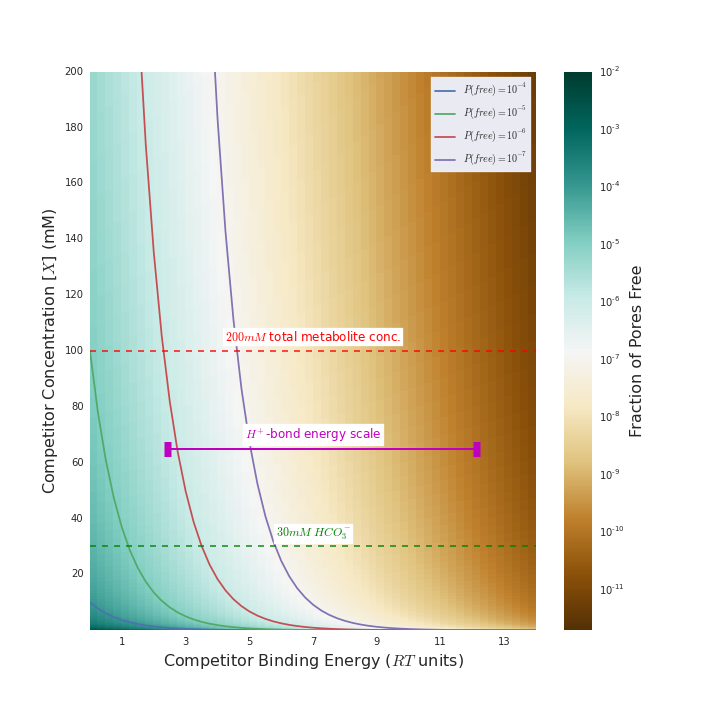
\includegraphics[scale=0.6]{figures/competitive_pore_energy_v_conc.png} 
\caption{The energetic scale of competitive interactions required to make the carboxysome '$CO_2$-tight.'}
\label{fig1}
\end{figure}

\subsection{Derivation for $HCO_3^-$ Entry}

Considering the case of $HCO_3^-$ entry, we must roll back our above assumption that $HCO_3^-$ and $X$ are in the same pool. As bicarbonate carries negative charge and can (presumably) interact with the pore, the definition of an empty pore is somewhat different in the case of $HCO_3^-$ than it was for $CO_2$. Since an $HCO_3^-$-bound pore can transit $HCO_3^-$, we now we define an empty pore as one not bound by $X$, rather than one that is entirely empty. We also "roll-back" the assumption that $HCO_3^-$ and $X$ have the same pore association energies - i.e. $\epsilon$ may be greater than $0$.  

\begin{align}
Pr(empty) = 1 - Pr(X bound) = 1 - \frac{[P^{free}][X]}{K_D^X [P^{total}]} \\
= 1 - \frac{[X]}{K_D^X \left( 1 + \frac{[HCO_3^{-free}]}{K_D^{HCO_3^-}} + \frac{[X^{free}]}{K_D^{X}}\right)} \\
= 1 - \frac{f}{\frac{K_D^X}{[HCO_3^-]} + f + \exp\left(-\epsilon / RT\right)}
\end{align}

where $f = \frac{[X]}{[HCO_3^-]}$ is the fold excess of competitor over $HCO_3^-$. Notice that this expression is independent of the absolute binding energy of $HCO_3^-$, $E_{HCO_3^-}$, and instead depends only on the absolute binding energy of the competitor $X$ and the difference in binding energy between $X$ and $HCO_3^-$, $\epsilon$. So while we must set $\epsilon$ and $E_{HCO_3^-}$ to calculate $Pr(empty)$, we need not fix $E_{HCO_3^-}$ explicitly (although its value is implicitly set by the other two). 

\begin{figure}[ht]
\centering
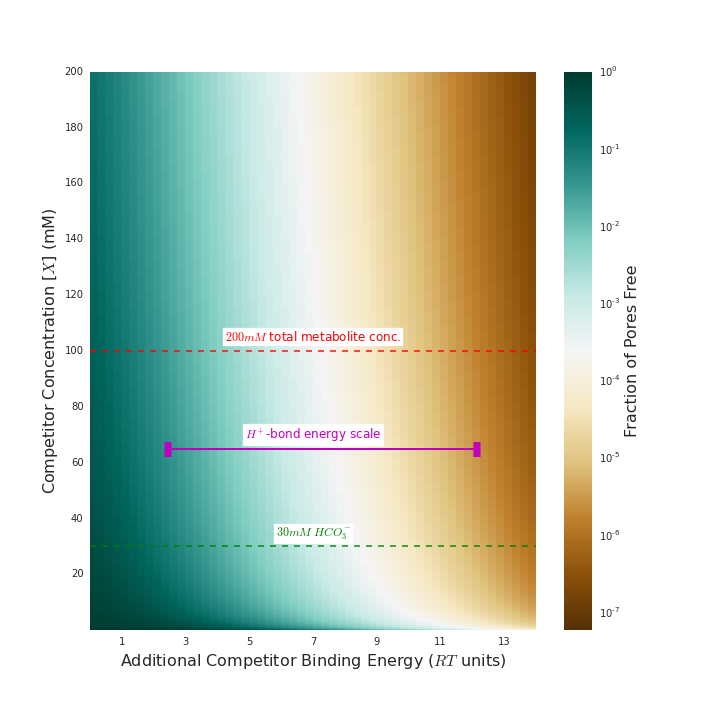
\includegraphics[scale=0.6]{figures/bicarbonate_competition.png} 
\caption{Since $HCO_3^-$ has a high ($\approx 30 mM$) concentration and can also bind the pore, competition from $X$ has a much smaller effect on it.}
\label{fig2}
\end{figure}

In ~\ref{fig2} we assumed a $E_{HCO_3^-} = 2.5 RT$ and calculated $Pr(free)$ for varying $\epsilon$ and $[X]$. Notice that this plot is essentially a rightward-shifted version of ~\ref{fig1}. 

\end{document}